\documentclass[a4paper,12pt]{article}
\usepackage[utf8]{inputenc}
\usepackage{geometry}
\usepackage{graphicx} 
\usepackage{listings} 
\usepackage{xcolor}
\usepackage{tikz}     
\usetikzlibrary{shapes, arrows, positioning, calc}


\geometry{left=2.5cm, right=2.5cm, top=2.5cm, bottom=2.5cm}


\definecolor{codegreen}{rgb}{0,0.6,0}
\definecolor{codegray}{rgb}{0.5,0.5,0.5}
\definecolor{codepurple}{rgb}{0.58,0,0.82}

\lstdefinestyle{mystyle}{
    backgroundcolor=\color{backcolour},   
    commentstyle=\color{codegreen},
    keywordstyle=\color{magenta},
    numberstyle=\tiny\color{codegray},
    stringstyle=\color{codepurple},
    basicstyle=\ttfamily\footnotesize,
    breakatwhitespace=false,         
    breaklines=true,                 
    captionpos=b,                    
    keepspaces=true,                 
    numbers=left,                    
    numbersep=5pt,                  
    showspaces=false,                
    showstringspaces=false,
    showtabs=false,                  
    tabsize=2
}
\lstset{style=mystyle}


\title{Practical Work 1: TCP File Transfer Report}
\author{
    \textbf{Nguyen Thanh Dat} \\ 
    Student ID: 23BI14091
}
\date{\today}

\begin{document}

\maketitle

\section{Introduction}
The goal of this practical work is to implement a one-to-one file transfer system using TCP/IP sockets within a Command Line Interface (CLI). This report details the design and implementation of the protocol used to reliably transfer files (specifically tested with \texttt{test.jpg}) between a client and a server.

\section{Protocol Design}
To ensure that the server knows exactly what file is arriving and how large it is, I designed a simple application-layer protocol.

\subsection{Protocol Logic}
\begin{enumerate}
    \item \textbf{Metadata Exchange:} Before sending the actual file content, the client sends a metadata header containing the \texttt{filename} and the \texttt{filesize} separated by a delimiter (\texttt{|}).
    \item \textbf{Data Stream:} Once the server parses the size, the client streams the bytes. The server reads exactly the number of bytes specified in the header.
\end{enumerate}

\subsection{Protocol Sequence Diagram}
\begin{center}
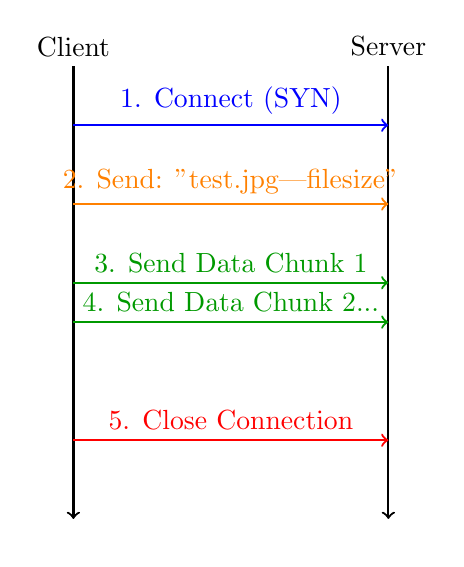
\begin{tikzpicture}[node distance=4cm, auto, thick]
    % Nodes
    \node (client) {Client};
    \node (server) [right of=client] {Server};
    
    % Lines representing time
    \draw [->] (client) -- (client |- 0,-6) node[below] {};
    \draw [->] (server) -- (server |- 0,-6) node[below] {};
    
    % Interactions
    \draw [->, blue] ($(client)+(0,-1)$) -- node [midway, above] {1. Connect (SYN)} ($(server)+(0,-1)$);
    \draw [->, orange] ($(client)+(0,-2)$) -- node [midway, above] {2. Send: "test.jpg|filesize"} ($(server)+(0,-2)$);
    \draw [->, green!60!black] ($(client)+(0,-3)$) -- node [midway, above] {3. Send Data Chunk 1} ($(server)+(0,-3)$);
    \draw [->, green!60!black] ($(client)+(0,-3.5)$) -- node [midway, above] {4. Send Data Chunk 2...} ($(server)+(0,-3.5)$);
    \draw [->, red] ($(client)+(0,-5)$) -- node [midway, above] {5. Close Connection} ($(server)+(0,-5)$);
    
\end{tikzpicture}
\captionof{figure}{Sequence Diagram of the File Transfer Protocol}
\end{center}

\section{System Organization}
The system consists of a single server and a single client. The server binds to a specific IP and Port and listens for incoming TCP requests. The client initiates the connection using a blocking socket.

\begin{center}
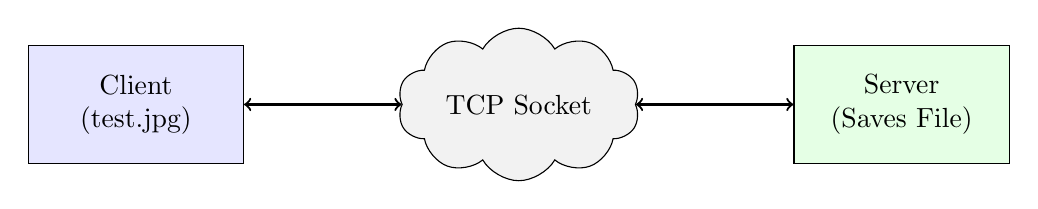
\begin{tikzpicture}[auto, node distance=2cm]
    \node [rectangle, draw, fill=blue!10, text width=2.5cm, align=center, minimum height=1.5cm] (cli) {Client\\(test.jpg)};
    \node [cloud, draw, cloud puffs=10, cloud puff arc=120, aspect=2, fill=gray!10, right=of cli] (net) {TCP Socket};
    \node [rectangle, draw, fill=green!10, text width=2.5cm, align=center, minimum height=1.5cm, right=of net] (srv) {Server\\(Saves File)};
    
    \draw [<->, thick] (cli) -- (net);
    \draw [<->, thick] (net) -- (srv);
\end{tikzpicture}
\captionof{figure}{System Architecture}
\end{center}

\section{Implementation}
The following is the core logic used to implement the file transfer.

\subsection{Client Side}
The client locates \texttt{test.jpg}, calculates its size, sends the header, and then streams the file content.
\begin{lstlisting}[language=Python]
filename = "test.jpg"
filesize = os.path.getsize(filename)

s.connect((HOST, PORT))

# 1. Send Metadata
metadata = f"{filename}|{filesize}"
s.sendall(metadata.encode())

# 2. Send File Content
with open(filename, 'rb') as f:
    while True:
        bytes_read = f.read(1024)
        if not bytes_read:
            break 
        s.sendall(bytes_read)
\end{lstlisting}

\subsection{Server Side}
The server receives the metadata, splits them to get the file size, and loops until it has received the total expected bytes.
\begin{lstlisting}[language=Python]
# 1. Receive Metadata
data = conn.recv(1024).decode()
filename, filesize = data.split('|')
filesize = int(filesize)

# 2. Receive File Data
received_bytes = 0
with open(filename, 'wb') as f:
    while received_bytes < filesize:
        chunk = conn.recv(1024)
        if not chunk:
            break
        f.write(chunk)
        received_bytes += len(chunk)
\end{lstlisting}


\end{document}